\element{EM2.sym}{
  \begin{question}{symB}\bareme{1}
    Le champ magnétique est inclus dans les plans
    \begin{multicols}{2}
      \begin{reponses}
        \bonne{d'antisymétrie}
        \mauvaise{de symétrie}
      \end{reponses}
    \end{multicols}
  \end{question}
}
\element{EM2.sym}{
  \begin{question}{antisymB}\bareme{1}
    Le champ magnétique est orthogonal aux plans
    \begin{multicols}{2}
      \begin{reponses}
        \bonne{de symétrie}
        \mauvaise{d'antisymétrie}
      \end{reponses}
    \end{multicols}
  \end{question}
}
\setgroupmode{EM2.sym}{cyclic}


\element{EM2.Ampere}{
  \begin{question}{thAmpere}\bareme{1}
    Le théorème d'Ampère s'écrit
    \begin{multicols}{2}
      \begin{reponses}
        \bonne{$\oint \vv{B}.\vv{dl}=\mu_0I_\text{enlacé}$}
        \mauvaise{$\oiint \vv{B}.\vv{dS}=\mu_0I_\text{enlacé}$}
        \mauvaise{$\oiint \vv{B}.\vv{dS}=\frac{I_\text{enlacé}}{\mu_0}$}
        \mauvaise{$\iiint B.dV=\mu_0\frac{I_\text{enlacé}}{\mu_0}$}
      \end{reponses}
    \end{multicols}
  \end{question}
}

\element{EM2.CourbeAmpere}{
  \begin{questionmult}{courbeAmpere}\bareme{haut=2,p=0}
    Dans l'exemple ci-dessous, la courbe d'Ampère, orientée dans le sens conventionnel par rapport à $I$

    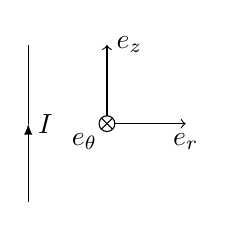
\begin{tikzpicture}
      \draw[->, >=latex] (0,0) -- (0,1) node[right] {$I$};
      \draw (0,1) -- (0,2);
      \draw[->] (1,1) -- (2,1) node[below] {$\vv{e_r}$};
      \draw[->] (1,1) -- (1,2) node[right] {$\vv{e_z}$};
      \draw[fill=white] (1,1) circle (0.1);
      \draw (1,1) ++(45:0.1) --++(-135:0.2);
      \draw (1,1) ++(-45:0.1) --++(135:0.2);
      \draw (1,1) node[below left] {$\vv{e_\theta}$};
    \end{tikzpicture}
    \begin{multicols}{2}
      \begin{reponses}
        \bonne{est fermée.}
        \bonne{est orientée selon $\vv{e_\theta}$.}
        \bonne{enlace le courant $I$.}
        \bonne{est un cercle.}
        \mauvaise{est orientée selon $\vv{e_r}$.}
        \mauvaise{est orientée selon $\vv{e_z}$.}
        \mauvaise{est un rectangle.}
        \mauvaise{est une sphère.}
      \end{reponses}
    \end{multicols}
  \end{questionmult}
}